\section{Introduction}
Virtualization-based server consolidation is a common practice in  today's cloud data 
centers \cite{ec2, azure, gcp}. Hypervisors host multiple
virtual machines (VMs), or guests, on a  single physical host to achieve benefits such as 
improved utilization  (hence, better return-on-investment) and agility in 
resource provisioning required for modern cloud applications~\cite{gcp_auto,heap_auto,azure_auto,gcp_serverless, lambdamodel}. 
Hypervisors must be often updated or replaced for various 
purposes, such as for applying security/bug fixes~\cite{xenpatch,kvmbugs}
adding new features~\cite{brasser2014swap, gcpsecurity},
or simply for software rejuvenation~\cite{le2011rehype}
to reset the effects of any unknown memory leaks or other latent bugs.

Updating a hypervisor or OS usually requires a system reboot, especially in 
the cases of system failures and software aging. 
Live patching \cite{Livepatch:Xen} can be used to perform
some of these updates without rebooting, but it relies greatly on 
the old hypervisor being patched, which can be buggy and unstable.
%TODO:Kartik: We also rely on the hypervisor being replaced, but less so. State this somewhere.
To eliminate the need for a system reboot and 
mitigate service disruption, another approach is to live migrate the VMs from the current host to another host that 
runs the clean and updated hypervisor.
Though widely used, live migrating~\cite{clark2005live, postcopy} tens or hundreds of 
VMs from one physical host to another, i.e. {\em inter-host live migration}, 
can lead to significant service disruption, long
total migration time, and large migration-triggered network traffic, which can
also affect other unrelated VMs~\cite{mann2012remedy}.

%We propose a faster and less disruptive approach to  
%live hypervisor replacement by leveraging nested virtualization and {\em intra-host live migration}.
In this paper, we present {\bf \arch}, a faster and less disruptive
approach to live hypervisor replacement which transparently
and quickly replaces an old hypervisor with a new instance on the same host
while minimizing runtime overheads on running VMs.
Using nested virtualization~\cite{turtles}, a lightweight shim layer, called 
the {\em hyperplexor}, runs beneath the traditional full-fledged hypervisor on which VMs run.
The new replacement hypervisor is instantiated as a guest atop the hyperplexor.
Next, the states of all VMs are transferred from the stale hypervisor to the
replacement hypervisor via intra-host live VM migration. 

Unfortunately, two major challenges must be tackled with this approach.
First, existing live migration techniques~\cite{clark2005live,postcopy} 
incur significant memory copying overhead, even for intra-host VM transfers.
Secondly, nested virtualization can degrade a VM's performance during
normal execution of VMs when no hypervisor replacement is being performed.
\arch addresses these two challenges as follows.

First, instead of copying the VM's
memory, the hyperplexor relocates the ownership 
of VM's memory pages from the old hypervisor to the 
new hypervisor.
%via a new data structure: {\em \arch table}. 
The hyperplexor records the mappings 
from VM's guest-physical and host-physical address space 
from the old hypervisor and uses them to reconstruct the 
VM's memory mappings on the replacement hypervisor. 
Most of the remapping operations are performed out of 
the critical path of the VM state transfer,
leading to very low hypervisor replacement times
of around 10ms, irrespective of the size of
the VMs being relocated. In contrast, traditional
intra-host VM migration, involving memory copying,
can take several seconds.
% -- 0.3 seconds for an idle 
%1 GB VM and 0.7 seconds for a busy write-intensive 1 GB VM,
%increasing linearly for larger VM sizes.
For the same reason, \arch also scales
well when remapping multiple VMs to the replacement
hypervisor.


%\arch leverages nested virtualization~\cite{turtles} to insert a lightweight 
%{\em hyperplexor} layer beneath the  traditional full-fledged hypervisor on which VMs 
%run. For hypervisor replacement, the hyperplexor initializes a new  hypervisor instance alongside the 
%old running hypervisor. Then, instead of copying guest memory, the hyperplexor simply 
%transfers guest memory mappings from extended/nested page tables of the old hypervisor to 
%the new hypervisor, along with any  virtual processor (VCPU) and I/O states. 

%Under the nested setting, hypervisor rejuvenation in \arch can be viewed as 
%an intra-host live VM migration mechanism between the stale hypervisor and 
%its replacement. To reduce the overhead of traditional live VM migration, 
%\arch involves a novel intra-host live VM migration technique: \arch co-maps 
%the running guest's memory to the replacement hypervisor's address space, 
%thus bypassing the need to perform expensive copying of the entire guest memory 
%as required with traditional live migration. Instead, \arch's migration operation 
%simply transfers the control of VMs virtual CPUs (VCPUs) and virtual I/O 
%devices between the two hypervisors, making the whole live migration 
%extremely fast (e.g., less than 10 ms).

\arch addresses the second challenge of nesting overhead as follows.
In comparison with the traditional single-level virtualization setup, 
where the hypervisor directly controls the hardware,
nested virtualization introduces additional overheads,
especially for I/O virtualization.  Hence \arch includes a number 
of optimizations to minimize nesting overheads,
allowing the hypervisor and 
its VMs to execute mostly without hyperplexor intervention during 
normal operations.  Specifically, \arch uses direct device 
assignment (VT-d) for emulation-free I/O path to the hypervisor, 
dedicates physical CPUs to reduce scheduling overheads for the hypervisor,
reduces CPU utilization on hyperplexor by disabling the polling of hypervisor VCPUs and eliminates VM Exits due to %common VM exits from the hypervisor to hyperplexor, such as for CPU idling
external device interrupts.

%\arch builds upon our preliminary 
%results reported in an earlier workshop paper~\cite{hyperfresh_apsys}. Our new contributions 
%include: (1) a more efficient and generic mechanism, the \arch 
%table, to relocate VMs/containers memory maps across co-resident hypervisors/
%VMs which reduces replacement time by an order of magnitude (e.g., 
%from 100ms to 10ms); (2) techniques to minimize  nesting overhead via direct 
%device assignment for emulation-free I/O, reduction of VM Exits due 
%to idling vCPUs and external interrupts; and (3) more comprehensive performance evaluations.

Finally, as a lightweight alternative to VMs,
containers~\cite{gcpkubernetes, azureks, ibmkubernetes, vmwarepks}
can be used to consolidate multiple processes.
We demonstrate that the hyperplexor-based approach 
can also be applied for {\em live replacement of an operating system}
beneath containers and processes. 
Specifically, we show how sub-second live OS replacement can be performed
by using a combination of the hyperplexor-based memory remapping mechanism 
and a well-known process migration tool, CRIU~\cite{criu}.
In this case, the hyperplexor runs as a thin shim layer (hypervisor)
beneath a traditional OS, which now runs in a low-overhead VM. 
For live OS replacement, 
the hyperplexor provisions a new VM, running the replacement OS, on the same 
physical host and transfers process/container memory mappings 
obtained via the CRIU tool.

In the rest of this paper, we first demonstrate the quantitative overheads 
of VM migration-based hypervisor replacement, followed by the design, implementation, 
and evaluation of \arch for VMs and containers, and finally discussion of 
related work and conclusions.

%We further reduce the network I/O overhead by directly assigning the 
%physical Network Interface Card (NIC) to the hypervisor. 
%Due to direct device assignment to hypervisor, the VM Exits due to 
%network I/O to hyperplexor are eliminated. The direct device assignment 
%improves the performance of the hypervisor but incurs high CPU utilization 
%on host. The vCPUs are further pinned to CPUs to reduce the CPU utilization 
%on host. Our previous work, HyperFresh \cite{bagdi2017hyperfresh} proposed 
%a technique to proactively replace an old buggy hypervisor with new 
%hypervisor by co-mapping the memory and transferring the vCPU and I/O 
%state on a refresh operation using nested virtualization. However, the 
%paper does not address the overhead caused due to nested virtualization. 
%We further reduce the total migration time and downtime with very less 
%modifications to the existing code and additionally, address the overhead 
%caused due to nested virtualization.


%\begin{figure}[t!]
%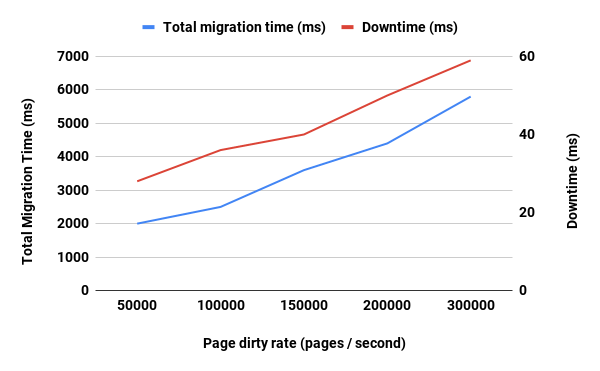
\includegraphics[width=0.5\textwidth]{figures/page_dirty_rate.png}
%\caption{Effect of page dirty rate on total migration time and downtime}
%\label{Effect of page dirty rate on total migration time and downtime}
%\end{figure}

%\begin{figure}[t!]
%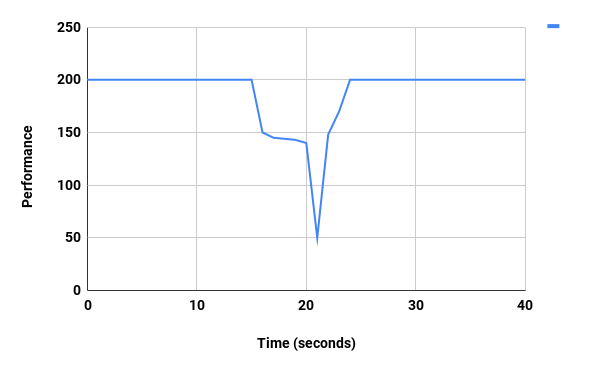
\includegraphics[width=0.5\textwidth]{figures/performance-10Gbps.png}
%\caption{Performance of X benchmark during migration over 10Gbps migration link %bandwidth}
%\label{Performance of X benchmark during migration over 10Gbps migration link bandwidth}
%\end{figure}

%\begin{figure}[t!]
%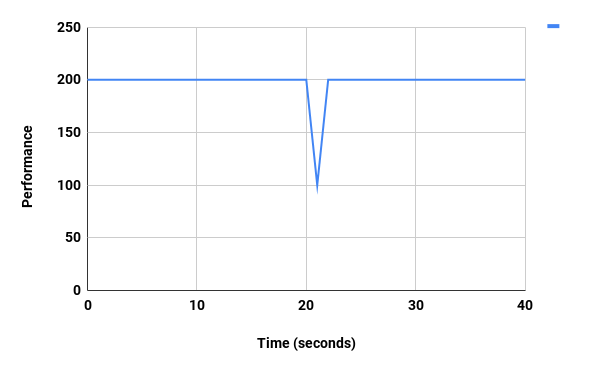
\includegraphics[width=0.5\textwidth]{figures/performance-40Gbps.png}
%\caption{Performance of X benchmark during migration over 40Gbps migration link %bandwidth}
%\label{Performance of X benchmark during migration over 40Gbps migration link bandwidth}
%\end{figure}


